%% ---------------------------------------------------------------------
%% 02 - CƠ SỞ LÝ THUYẾT
%% ---------------------------------------------------------------------

\section{Cơ sở lý thuyết}\label{sec:theory}

\subsection{Kiến thức miền}

Bề mặt đa diện tam giác hóa là bề mặt $P$ của một polytope trong $\R^3$ (khối đa
diện --- bản ba chiều của đa giác: lập phương, lăng trụ, \ldots), được chia thành
$n$ tam giác. Hai điểm $a,b$ trên $P$ nối với nhau bằng một đường nằm trọn trên
$P$; trong số mọi đường đó có đường ngắn nhất, ký hiệu $SP(a,b)$. Khi xét trong
một tập con $S$ của bề mặt, ký hiệu $SP_S(a,b)$ nghĩa là đường ngắn nhất
\emph{bị giới hạn trong} $S$ \cite{an2024funnel}. Nghiên cứu giới hạn ở trường
hợp polytope lồi (nối hai điểm bất kỳ bằng đoạn thẳng luôn nằm trong khối);
trường hợp không lồi đi theo cách xử lý tương ứng mà bài báo ghi chú là mở rộng.

Với một đường $\gamma$ trên bề mặt, tại mỗi điểm $w$ của $\gamma$ đo góc trái
$\alpha_{wl}$ và góc phải $\alpha_{wr}$; $\gamma$ được gọi là \emph{straightest
geodesic} (trắc địa thẳng nhất) khi hai góc này bằng nhau tại mọi $w$, tức khi
trải phẳng ra thì $\gamma$ thành một đoạn thẳng, không gấp khúc. Hai tính chất
được dùng về sau:
\begin{enumerate}
  \item Mọi đường ngắn nhất từ nguồn $s$ đến một đỉnh đều là \emph{straightest
    geodesic}.
  \item Vì đường trái của một phễu chính là $SP(s,p)$ nên nó tự động là
    \emph{straightest geodesic} --- đây là chi tiết quyết định cho toàn bộ thuật
    toán.
\end{enumerate}

Cho một dãy $m\ge 2$ tam giác liền kề $f_1,\ldots,f_m$ (gộp thành vùng $S$), một
đỉnh $s$ của $f_1$, hai đỉnh $p,q$ ở hai đầu dãy sao cho khi nhìn theo hướng
$f_1\to f_m$ thì $SP(s,p)$ nằm bên trái $SP(s,q)$. Funnel $F_{p,q,S}$ là vùng $S$
bị giới hạn bởi ba đường $SP(s,p)\cup SP(s,q)\cup SP(p,q)$ \cite{an2024funnel}.
Các thành phần của phễu được liệt kê trong Bảng~\ref{tab:thanh-phan-funnel}.

\begin{table}[!t]
  \caption{Các thành phần của một phễu.}
  \label{tab:thanh-phan-funnel}
  {\fontsize{7}{9.3}\selectfont
  \begin{tabular}{@{}>{\raggedright\arraybackslash}p{58pt}>{\raggedright\arraybackslash}p{126pt}@{}}
    \toprule
    \textbf{Thuật ngữ} & \textbf{Ý nghĩa} \\
    \midrule
    Cusp (đỉnh chụm) $s$ & Gốc của phễu; với polytope lồi, hai biên chỉ giao nhau
      tại $s$ \\
    Left border $SP(s,p)$ & Biên trái; luôn là \emph{straightest geodesic} \\
    Right border $SP(s,q)$ & Biên phải \\
    Direct destination $v$ & Đỉnh nằm ngoài $S$ nhưng kề cạnh với $q$ --- đích mà
      phễu có thể ``vươn tới'' \\
    \bottomrule
  \end{tabular}}
\end{table}

Hình~\ref{fig:funnel-cusp} minh họa cấu trúc này bằng một sơ đồ phẳng: vùng tam
giác $S$ giữa hai biên, cusp $s$, hai biên $SP(s,p)$ và $SP(s,q)$, cùng cạnh
$[q,v]$ dẫn tới đỉnh đích $v$.

\begin{figure}[!t]
  \centering
  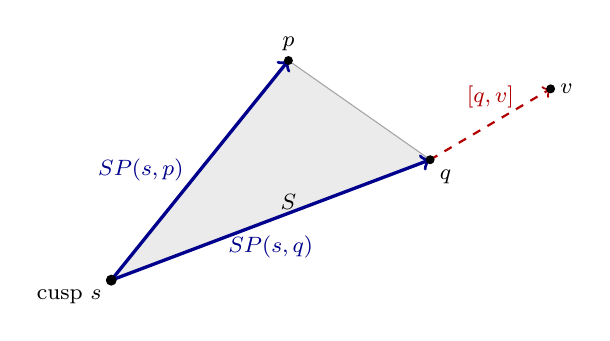
\begin{tikzpicture}[scale=0.9, every node/.style={font=\footnotesize}]
    \coordinate (s) at (0,0);
    \coordinate (p) at (2.5,3.1);
    \coordinate (q) at (4.5,1.7);
    \coordinate (v) at (6.2,2.7);
    \fill[black!8] (s) -- (p) -- (q) -- cycle;
    \draw[black!35] (p) -- (q);
    \draw[very thick, blue!55!black, ->] (s) -- (p)
      node[midway, left=2pt] {$SP(s,p)$};
    \draw[very thick, blue!55!black, ->] (s) -- (q)
      node[midway, below=2pt] {$SP(s,q)$};
    \draw[thick, red!70!black, dashed, ->] (q) -- (v)
      node[midway, above=2pt] {$[q,v]$};
    \fill (s) circle (2.2pt) node[below left] {cusp $s$};
    \fill (p) circle (1.8pt) node[above] {$p$};
    \fill (q) circle (1.8pt) node[below right] {$q$};
    \fill (v) circle (1.8pt) node[right] {$v$};
    \node at (2.5,1.1) {$S$};
  \end{tikzpicture}
  \caption{Cấu trúc phễu: cusp $s$, left border $SP(s,p)$, right border $SP(s,q)$
    và cạnh $[q,v]$ dẫn tới direct destination $v$. Đây là sơ đồ khái niệm, không
    phải ảnh kết quả từ repo.}
  \label{fig:funnel-cusp}
\end{figure}

Hình~\ref{fig:funnel-cusp} cho thấy vùng $S$ nằm giữa hai biên, cusp $s$ là nơi
hai biên gặp nhau, và cạnh $[q,v]$ là lối duy nhất để phễu vươn sang tam giác kề.
Khi phễu mở rộng, biên trái $SP(s,p)$ vẫn là đường trắc địa thẳng nhất; đây là
bất biến mà các bước so sánh góc và độ dài dựa vào.

Từ một phễu, khi mở rộng vùng $S$ bằng các tam giác kề cạnh $[q,v]$ ta được các
phễu con (\emph{child}); quan hệ con -- cha này dựng nên một cây có gốc là $s$,
gọi là \textbf{funnel tree}. Mỗi nút của cây là một cặp (phễu, $SP_S(p,q)$); khi
cây hoàn chỉnh, mỗi đường ngắn nhất $SP(s,v)$ ứng với đúng một nút trong cây, nên
việc dựng cây đồng thời tính ra mọi đường ngắn nhất từ $s$ \cite{an2024funnel}.

Một cách tiếp cận truyền thống là trải phẳng (\emph{planar unfolding}): ``mở'' các
tam giác xuống mặt phẳng sao cho giữ nguyên chiều dài cạnh; trên mặt phẳng, đường
ngắn nhất là đoạn thẳng nên dễ tính bằng tọa độ. Nhược điểm là mỗi lần mở lại phải
chuỗi theo một loạt phép biến hình đẳng cự, và khi cửa sổ (\emph{window}) di
chuyển qua các tam giác thì phải cập nhật lại. Toàn bộ nhánh Chen -- Han dùng kỹ
thuật này.

\subsection{Cơ sở khoa học dữ liệu}

Nghiên cứu không có mô hình học máy để huấn luyện: không có tập huấn luyện, tập
kiểm thử và không dự đoán nhãn. Vì vậy phần ``khoa học dữ liệu'' nằm ở quy trình
đo lường và kiểm chứng, tương tự một thực nghiệm tính toán (\emph{computational
experiment}):
\begin{description}
  \item[Dữ liệu vào] bộ mesh --- mỗi mesh là một tập cấu trúc (tập đỉnh, tập mặt,
    quan hệ kề), sinh bằng mã nguồn trong nghiên cứu; đặc trưng của từng mesh (số
    đỉnh, số mặt, độ cao, số cạnh biên) được mô tả ở Mục~\ref{sec:data}.
  \item[Biến đo được] độ dài đường đi $|SP(s,v)|$, sai số tương đối so với
    reference, số lần lan truyền $P$, thời gian chạy và các sai số bám tuyến từ
    telemetry.
  \item[Chuẩn đối chiếu] vì đây là bài toán có đáp án chính xác, ``nhãn'' thay thế
    bằng các polyline tham chiếu độc lập cho 5 mesh nhỏ. Bốn mesh không có reference và bề mặt thành phố không có bộ giải độc lập
    trong repo, nên chỉ được kiểm tra khả năng chạy và tính nhất quán nội tại.
    Quy trình: sinh mesh $\to$ chạy thuật toán $\to$ đối chiếu độ dài với reference
    $\to$ tổng hợp thành bảng số liệu.
\end{description}

Cách đặt này cũng giải thích vì sao các chỉ số quen thuộc của bài toán phân loại
(Accuracy, F1, ROC-AUC) \textbf{không áp dụng} ở đây: không tồn tại dự đoán sai
lệch xác suất để đo, chỉ có sai số giữa hai giá trị số thực.

\subsection{Các thuật toán sử dụng}

Theo Phan, Hoai và Thinh, nhánh phương pháp Chen và Han duy trì các cửa sổ trên bề
mặt đã trải phẳng và lan truyền chúng qua các mặt kề nhau; đây là cơ sở để bài
báo đối sánh với Funnel Tree \cite{an2024funnel}.

Thuật toán chính của bài báo \cite{an2024funnel} thay bước trải phẳng bằng
\textbf{so sánh góc trực tiếp trên khối ba chiều}, nhờ hai dữ kiện ở mục trên:
left border là \emph{straightest geodesic}, nên hình học của phễu xác định được
bằng định luật cos
\begin{equation}
  c=\sqrt{a^2+b^2-2ab\cos\theta}.
  \label{eq:cosine}
\end{equation}
Thuật toán gồm hai phần:
\begin{itemize}
  \item \textbf{Algorithm 1 (dựng cây):} từ cusp $s$, cây lớn dần theo từng tầng.
    Với mỗi phễu $F_{p,q,S}$ và mỗi direct destination $v$, tính góc $\beta_v$
    bằng \eqref{eq:cosine} rồi rẽ nhánh theo hai điều kiện: (5) $\beta_v<\pi$ ---
    nếu không thỏa thì phần trong của phễu con rỗng và dừng lại; (6)
    $\angle psv<\angle psw$ --- nếu thỏa thì sinh hai con, không thì một con. Mỗi
    phễu chỉ tốn $O(1)$ phép so sánh, tổng số nút của cây là $O(n^2)$ nên độ phức
    tạp thời gian và bộ nhớ đều là $O(n^2)$.
  \item \textbf{Thủ tục 2 (clip off funnels):} xử lý trường hợp hai phễu cùng cusp
    cùng ``chiếm'' một đỉnh (\emph{occupy a vertex}) --- khi đó đỉnh đó bị loại ra
    khỏi cây cho đến khi phễu được mở rộng đầy đủ rồi mới gán lại, để duy trì tính
    đúng đắn và giới hạn số nút. Trong thực tế các đỉnh bị loại rất ít.
\end{itemize}
Trong cài đặt, mỗi nút của cây lưu một bộ ba số $(x,y,z)$ lần lượt là góc tại
cusp, độ dài left border $|sp|$ và góc $\angle spq$ \cite{an2024funnel} --- chính
ba đại lượng mà \eqref{eq:cosine} cần.

Ba đoạn mã dưới đây là lõi của Thuật toán 1 và Thủ tục 2 trong cài đặt Python của
nghiên cứu \cite{quangnguyen2025} ($\beta_v$, $\angle psv$, $\angle pvw$ là các
đại lượng ký hiệu như trong bài báo): Mã~\ref{code:alg1} dựng cây theo từng tầng
(đúng dòng 5--18 của Thuật toán 1), Mã~\ref{code:alg1-expand} là phần mở rộng
từng phễu --- nơi chứa các điều kiện rẽ nhánh (5) và (6), và Mã~\ref{code:clip2}
triển khai Thủ tục 2.

\begin{code}[!t]
  \lstinputlisting[style=pycode]{Code/funnel_tree.py}
  \caption{Thuật toán 1 (\texttt{funnel\_tree.py}): dựng funnel tree gốc $s$.}
  \label{code:alg1}
\end{code}

\begin{code}[!t]
  \lstinputlisting[style=pycode]{Code/funnel_expand.py}
  \caption{Thuật toán 1 (\texttt{funnel\_expand.py}): mở rộng một phễu.}
  \label{code:alg1-expand}
\end{code}

\begin{code}[!t]
  \lstinputlisting[style=pycode]{Code/funnel_clip.py}
  \caption{Thủ tục 2 (\texttt{funnel\_clip.py}): clip off funnels.}
  \label{code:clip2}
\end{code}

Sau khi lan truyền, polyline ứng viên được tái dựng bằng cách trải phẳng dải mặt
đã chọn; đây là một khác biệt cần nêu rõ so với mục tiêu xử lý hoàn toàn nội tại
trong phương pháp gốc. Đối với bề mặt có cấu hình không lồi, bản triển khai xét
thêm các nguồn phụ tại những đỉnh có tổng góc mặt vượt $2\pi$ theo ngưỡng số của
chương trình, rồi ghép các đoạn đường giữa nguồn và đích thông qua một đồ thị có
trọng số. Đồ thị này được tìm kiếm bằng A* với heuristic
$h(v)=\norm{v-g}$; khoảng cách thẳng trong $\R^3$ là cận dưới cho độ dài một đường
bị ràng buộc nằm trên bề mặt, nên A* chỉ dùng để chọn các đoạn ứng viên trong đồ
thị nguồn phụ, không thay bề mặt bằng đồ thị cạnh tam giác đơn thuần. Sau tái dựng,
chương trình kiểm tra đường thuộc lưới và kiểm tra tính nhất quán giữa độ dài lan
truyền với độ dài polyline. Việc tìm được đường trên đồ thị nguồn phụ chưa tự
chứng minh đường đó tối ưu trên toàn bề mặt; bước đối chiếu với chương trình tham
chiếu được thực hiện riêng.

Bảng~\ref{tab:chenhan-vs-funnel} tóm tắt đối sánh hai nhánh theo bài báo gốc
\cite{an2024funnel}.

\begin{table}[!t]
  \caption{So sánh nhóm Chen -- Han và funnel tree.}
  \label{tab:chenhan-vs-funnel}
  {\fontsize{7}{8.6}\selectfont
  \begin{tabular}{@{}>{\raggedright\arraybackslash}p{48pt}>{\raggedright\arraybackslash}p{66pt}>{\raggedright\arraybackslash}p{66pt}@{}}
    \toprule
    \textbf{Tiêu chí} & \textbf{Chen và Han (1996)} & \textbf{Funnel tree (2024)} \\
    \midrule
    Độ phức tạp & $O(n^2)$ & $O(n^2)$ \\
    Trải phẳng & Có --- mỗi cửa sổ một chuỗi phép biến hình & Không --- so sánh
      góc bằng định luật cos trên ba chiều \\
    Nguồn ảnh, phép chiếu & Có & Không \\
    Kỹ thuật & Lan truyền cửa sổ trên mặt phẳng & Phễu và \emph{straightest
      geodesic} \\
    Số nút trên \texttt{cube4} & \num{1287379} & \num{10401} \\
    Hiệu năng thực nghiệm & Tham chiếu & Nhanh hơn 1 đến 12 lần \\
    \bottomrule
  \end{tabular}}
\end{table}

Funnel tree được chọn vì ba lý do: (i) cây một nguồn -- mọi đích trùng khớp trực
tiếp với yêu cầu kho -- mọi khách; (ii) cùng độ phức tạp $O(n^2)$ nhưng ít phép
toán hơn; (iii) cài đặt bằng Python gọn, chỉ cần NumPy cho mảng và thư viện chuẩn,
không cần thư viện hình học. Kết quả cài đặt được đối chiếu với các đầu ra tham
chiếu đi kèm bộ mã nguồn của nghiên cứu \cite{quangnguyen2025}.

\subsection{Chỉ số đánh giá}

Vì là bài toán tìm đường đúng -- sai, các chỉ số là các đại lượng số thực giữa đáp
án của thuật toán và giá trị tham chiếu, được liệt kê trong
Bảng~\ref{tab:chi-so-danh-gia}.

\begin{table*}[!t]
  \caption{Các chỉ số đánh giá.}
  \label{tab:chi-so-danh-gia}
  {\fontsize{7}{8.6}\selectfont
  \setlength{\tabcolsep}{4pt}%
  \begin{tabular}{@{}>{\raggedright\arraybackslash}p{70pt}>{\raggedright\arraybackslash}p{160pt}>{\raggedright\arraybackslash}p{150pt}@{}}
    \toprule
    \textbf{Chỉ số} & \textbf{Định nghĩa} & \textbf{Vai trò} \\
    \midrule
    Độ dài đường đi & $\norm{SP(s,v)}$ --- độ dài đường ngắn nhất trên bề mặt &
      kết quả chính của thuật toán \\
    \addlinespace
    Sai số tương đối & $\varepsilon=\bigl|\,\norm{SP}-d_{\text{ref}}\,\bigr|/d_{\text{ref}}$
      so với đường tham chiếu & đối chiếu 5 mesh có reference \\
    \addlinespace
    Số lần lan truyền & $P$ --- số lần gọi \texttt{propagate} trong một lượt tìm &
      đo quy mô tìm kiếm \\
    \addlinespace
    Thời gian lập tuyến & giây, gồm đọc mesh và ghi JSON & số liệu quan sát, không
      dùng làm benchmark \\
    \addlinespace
    Sai số bám tuyến & $e_{\max}$, $\bar e$, $e_{\rm final}$ từ telemetry &
      đánh giá chuyến bay \\
    \addlinespace
    Hợp lệ / đạt mốc & hết tuyến và $e_{\rm final}\le0{,}5$ / thêm
      $e_{\max}\le1{,}0$ & hai tiêu chí tách riêng \\
    \bottomrule
  \end{tabular}}
\end{table*}

Sai số tương đối với chuẩn, khi cần, được tính theo
$\varepsilon=\bigl|\,\norm{SP}-d_{\text{chuẩn}}\,\bigr|/d_{\text{chuẩn}}$. Các
chỉ số Accuracy, Precision, Recall, F1, ROC-AUC \emph{không} được dùng vì không
có tập dự đoán phân loại.
